\documentclass[10pt]{beamer}
\usetheme[
%%% options passed to the outer theme
%    hidetitle,           % hide the (short) title in the sidebar
%    hideauthor,          % hide the (short) author in the sidebar
%    hideinstitute,       % hide the (short) institute in the bottom of the sidebar
%    shownavsym,          % show the navigation symbols
%    width=2cm,           % width of the sidebar (default is 2 cm)
%    hideothersubsections,% hide all subsections but the subsections in the current section
%    hideallsubsections,  % hide all subsections
%    left                % right of left position of sidebar (default is right)
  ]{Aalborg}
  
% If you want to change the colors of the various elements in the theme, edit and uncomment the following lines
% Change the bar and sidebar colors:
%\setbeamercolor{Aalborg}{fg=red!20,bg=red}
%\setbeamercolor{sidebar}{bg=red!20}
% Change the color of the structural elements:
%\setbeamercolor{structure}{fg=red}
% Change the frame title text color:
%\setbeamercolor{frametitle}{fg=blue}
% Change the normal text color background:
%\setbeamercolor{normal text}{bg=gray!10}
% ... and you can of course change a lot more - see the beamer user manual.

\usepackage[utf8]{inputenc}
\usepackage[spanish]{babel}
\usepackage[T1]{fontenc}
% Or whatever. Note that the encoding and the font should match. If T1
% does not look nice, try deleting the line with the fontenc.

\usepackage[table,xcdraw]{xcolor}
\usepackage{helvet}
\usepackage{tikz}
\usetikzlibrary{shapes,arrows,positioning}

\usepackage{minted}


\usepackage{listings}
\usepackage{color}
\definecolor{codegreen}{rgb}{0,0.6,0}
\definecolor{codegray}{rgb}{0.5,0.5,0.5}
\definecolor{codepurple}{rgb}{0.58,0,0.82}
\definecolor{backcolour}{rgb}{0.95,0.95,0.92}
 
\lstdefinestyle{mystyle}{
    backgroundcolor=\color{backcolour},   
    commentstyle=\color{codegreen},
    keywordstyle=\color{magenta},
    numberstyle=\tiny\color{codegray},
    stringstyle=\color{codepurple},
    basicstyle=\footnotesize,
    breakatwhitespace=false,         
    breaklines=true,                 
    captionpos=b,                    
    keepspaces=true,                 
    numbers=left,                    
    numbersep=5pt,                  
    showspaces=false,                
    showstringspaces=false,
    showtabs=false,                  
    tabsize=2
}
 
\lstset{style=mystyle}


% colored hyperlinks
\newcommand{\chref}[2]{%
  \href{#1}{{\usebeamercolor[bg]{Aalborg}#2}}%
}

\title[Servomecanismos]% optional, use only with long paper titles
{Servomecanismos}

\subtitle{Git y Github para poetas, parte 3}  % could also be a conference name

\date{\today}

\author[Víctor Medrano Zarazúa] % optional, use only with lots of authors
{
  Víctor Medrano Zarazúa\\
  \href{mailto:victor.medranozr@uanl.edu.mx}{{\tt victor.medranozr@uanl.edu.mx}}
}
% - Give the names in the same order as they appear in the paper.
% - Use the \inst{?} command only if the authors have different
%   affiliation. See the beamer manual for an example

\institute[
%  {\includegraphics[scale=0.2]{aau_segl}}\\ %insert a company, department or university logo
  %Dept.\ of Electronic Systems\\
  Universidad Autónoma de Nuevo León\\
  Facultad de Ingeniería Mecánica y Eléctrica
] % optional - is placed in the bottom of the sidebar on every slide
{% is placed on the bottom of the title page
  %Department of Electronic Systems\\
  Universidad Autónoma de Nuevo León\\
  Facultad de Ingeniería Mecánica y Eléctrica
  
  %there must be an empty line above this line - otherwise some unwanted space is added between the university and the country (I do not know why;( )
}

% specify the logo in the top right/left of the slide
\pgfdeclareimage[height=1cm]{mainlogo}{AAUgraphics/FIME} % placed in the upper left/right corner
\logo{\pgfuseimage{mainlogo}}

% specify a logo on the titlepage (you can specify additional logos an include them in 
% institute command below
\pgfdeclareimage[height=1.5cm]{titlepagelogo}{AAUgraphics/UANL} % placed on the title page
%\pgfdeclareimage[height=1.5cm]{titlepagelogo2}{AAUgraphics/aau_logo_new} % placed on the title page
\titlegraphic{% is placed on the bottom of the title page
  \pgfuseimage{titlepagelogo}
%  \hspace{1cm}\pgfuseimage{titlepagelogo2}
}

%\definecolor{UniBlue}{RGB}{255,255,255}

\tikzset{
block/.style={
  draw, 
  fill=blue!20, 
  rectangle, 
  minimum height=3em, 
  minimum width=6em
  },
 gain/.style={
    draw,
    fill=blue!20, 
    isosceles triangle,
    minimum height = 3em,
    isosceles triangle apex angle=60
    },
sum/.style={
  draw, 
  fill=blue!20, 
  circle, 
  },
input/.style={coordinate},
output/.style={coordinate},
pinstyle/.style={
  pin edge={to-,thin,black}
  }
}  

\begin{document}
% the titlepage


%\setbeamercolor{title}{fg=UniBlue}
%\setbeamercolor{normal text}{fg=UniBlue}
%\setbeamercolor{Aalborg}{fg=black,bg=black}


{\aauwavesbg
\begin{frame}[plain,noframenumbering] % the plain option removes the sidebar and header from the title page
  \titlepage
\end{frame}}
%%%%%%%%%%%%%%%%

% TOC
\begin{frame}{Contenido}{}
\tableofcontents
\end{frame}
%%%%%%%%%%%%%%%%
\section{Repaso}
\begin{frame}{Repaso}{}
\begin{block}{Recapítulemos...}
\begin{itemize}
    \item ¿Qué es un fork?
    \item ¿Cuáles son las diferentes formas de hacer un pull request?
\end{itemize}
\end{block}

%\begin{figure}[h!]
%\centering
%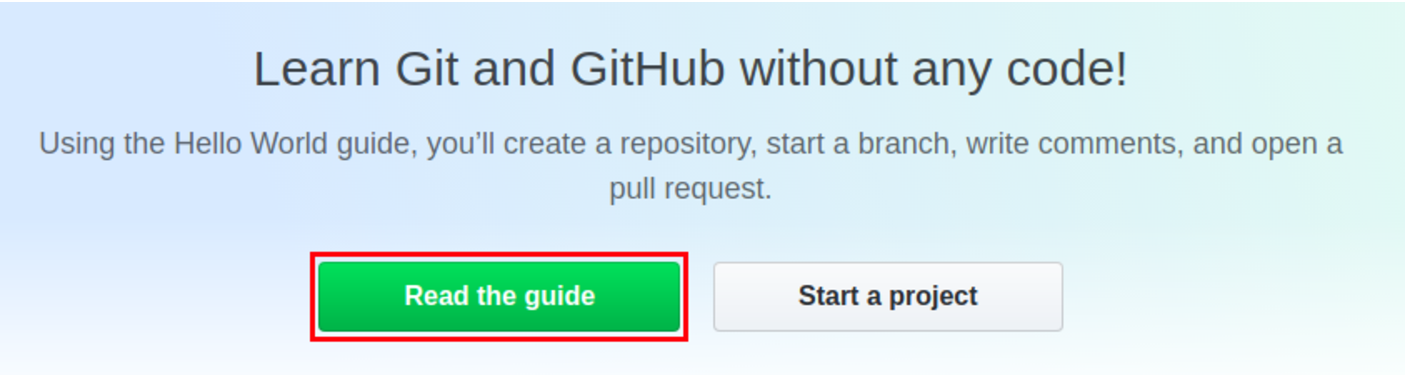
\includegraphics [scale=0.32]{github}
%\caption{Bobina Tesla}
%\label{fig:tesla}
%\end{figure}

\end{frame}

\section{Introducción}

\begin{frame}{Introducción}{}
\begin{block}{Prepáranse para los problemas...}
\medskip
\begin{columns}[c]
\column{1.5in}
\begin{itemize}
    \item Hablaremos de como registrar problemas que se presentan en nuestro poema (código) y cómo hacer referencia a un problema en particular cuando se hace un cambio (commit) a un archivo del repositorio.
\end{itemize}

\column{2in}
\framebox{
\includegraphics[width=2in]{james.jpg}}
\end{columns}
\end{block}
\end{frame}

\section{Issues}

\begin{frame}{Issues}{Problemas con el poema e ideas para mejorarlo}
\begin{block}{}

\begin{columns}[c]
\column{2.3in}
\vspace{-0.2in}
\begin{itemize}
        \item Los \textcolor{blue}{issues} no son propiamente un concepto del software Git como los que hemos visto anteriormente (repositorio, commits, branching, pull request, etc.)\\
        
        \item Los \textcolor{blue}{issues} existen como una característica integrada en la plataforma de Github. Estos fueron creados con el propósito de propiciar la colaboración dentro del sitio y juegan un rol vital dentro de el mismo; sobre todo en proyectos sumamente complejos.
\end{itemize}

\column{1.3in}
\framebox{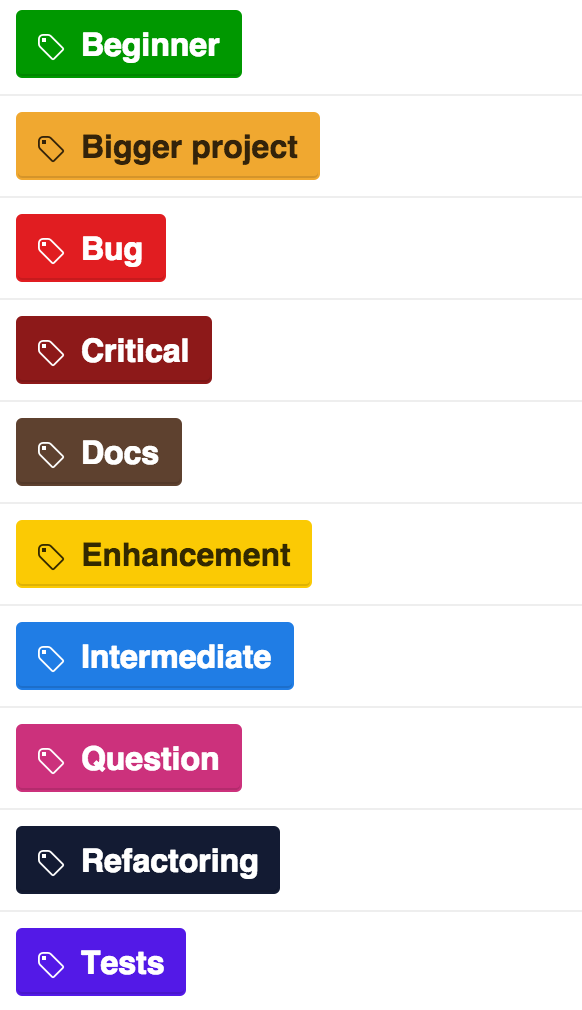
\includegraphics[width=1.3in]{issueslabels.png}}
\end{columns}
    
\end{block}

\end{frame}

\begin{frame}{Issues}{Problemas con el poema e ideas para mejorarlo}

\begin{block}{}

%\begin{columns}[c]
\begin{itemize}
        \item En pocas palabras, la sección de \textcolor{blue}{issues} es un lugar destinado a comentarios acerca de un proyecto (e.g: encontré un bug, escribí mal una palabra, tengo dudas acerca del código, etc.)
\end{itemize}

\begin{figure}[h!]
\centering
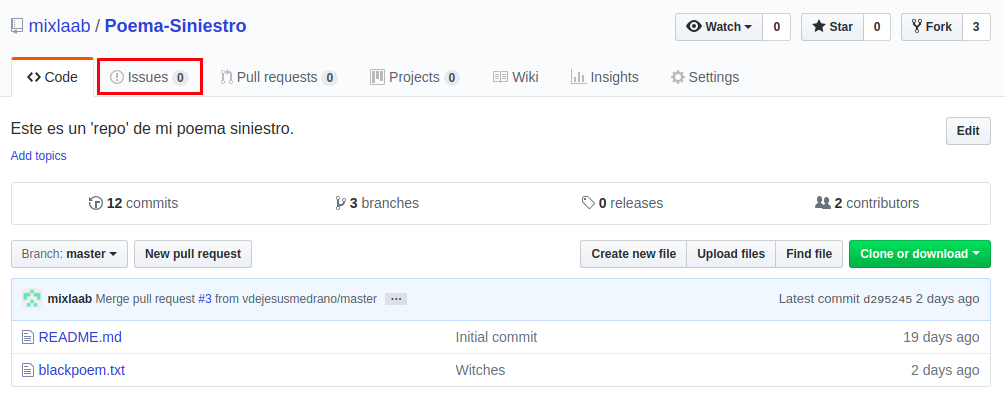
\includegraphics [scale=0.27]{issues}
%\caption{Sección de Issues}
\label{fig:issues}
\end{figure}
    
\end{block}

\end{frame}

\begin{frame}{Issues}{Problemas con el poema e ideas para mejorarlo}

\begin{block}{}
\vspace{-0.3in}
\begin{figure}[h!]
\centering
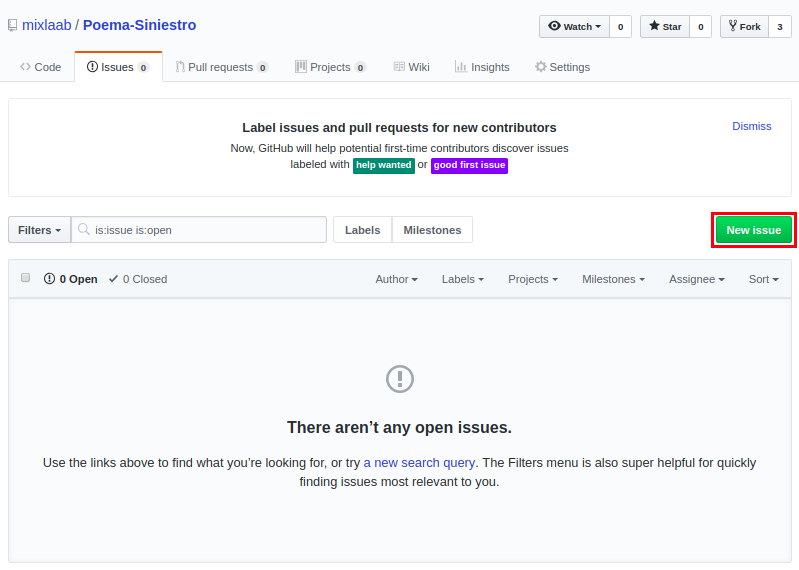
\includegraphics [scale=0.35]{newissue}
%\caption{Sección de Issues}
\label{fig:issues}
\end{figure}
    
\end{block}

\end{frame}

\begin{frame}{Issues}{Problemas con el poema e ideas para mejorarlo}

\begin{block}{Uso de Markdown}
\vspace{-0.15in}
\begin{figure}[h!]
\centering
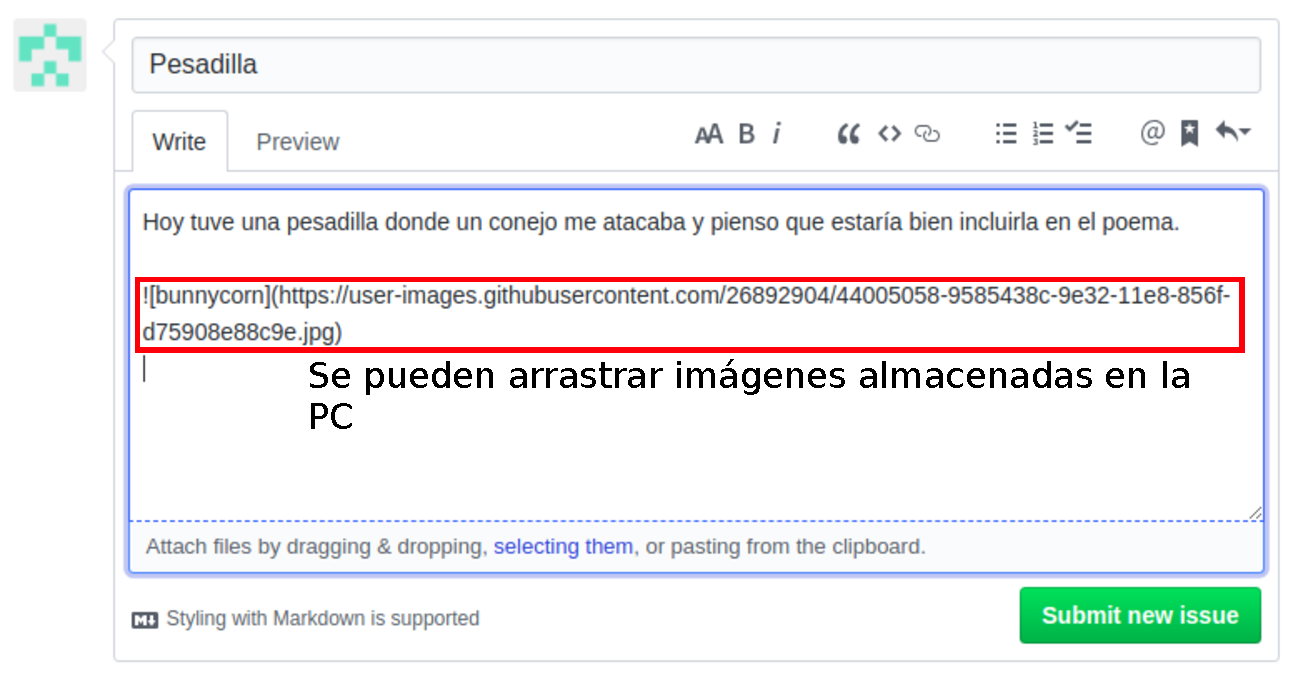
\includegraphics [scale=0.45]{nightmare}
%\caption{Sección de Issues}
\label{fig:images}
\end{figure}
    
\end{block}

\end{frame}

\begin{frame}{Issues}{Problemas con el poema e ideas para mejorarlo}

\begin{block}{Uso de Markdown}
\vspace{-0.15in}
\begin{figure}[h!]
\centering
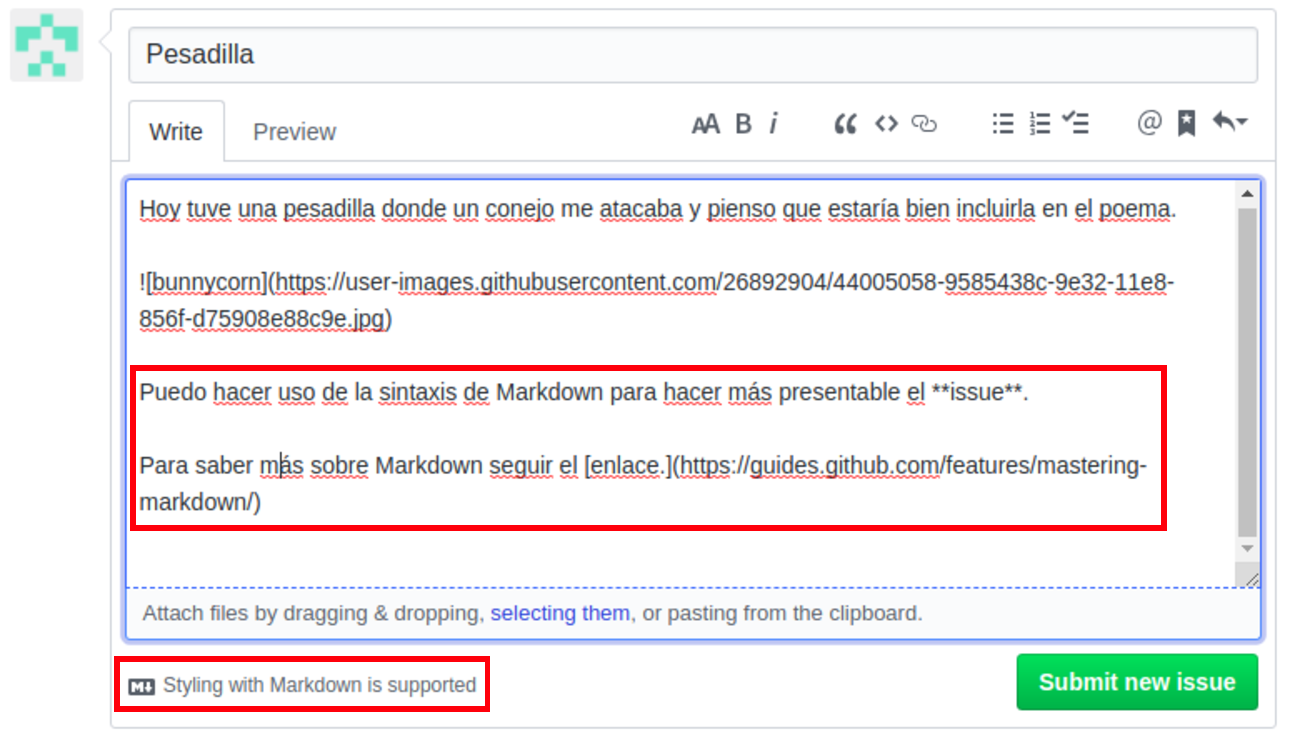
\includegraphics [scale=0.45]{markdown}
\label{fig:markdown}
\end{figure}
    
\end{block}

\end{frame}

\begin{frame}{Issues}{Problemas con el poema e ideas para mejorarlo}

\begin{block}{Uso de Markdown}
%\vspace{-0.15in}
\begin{figure}[h!]
\centering
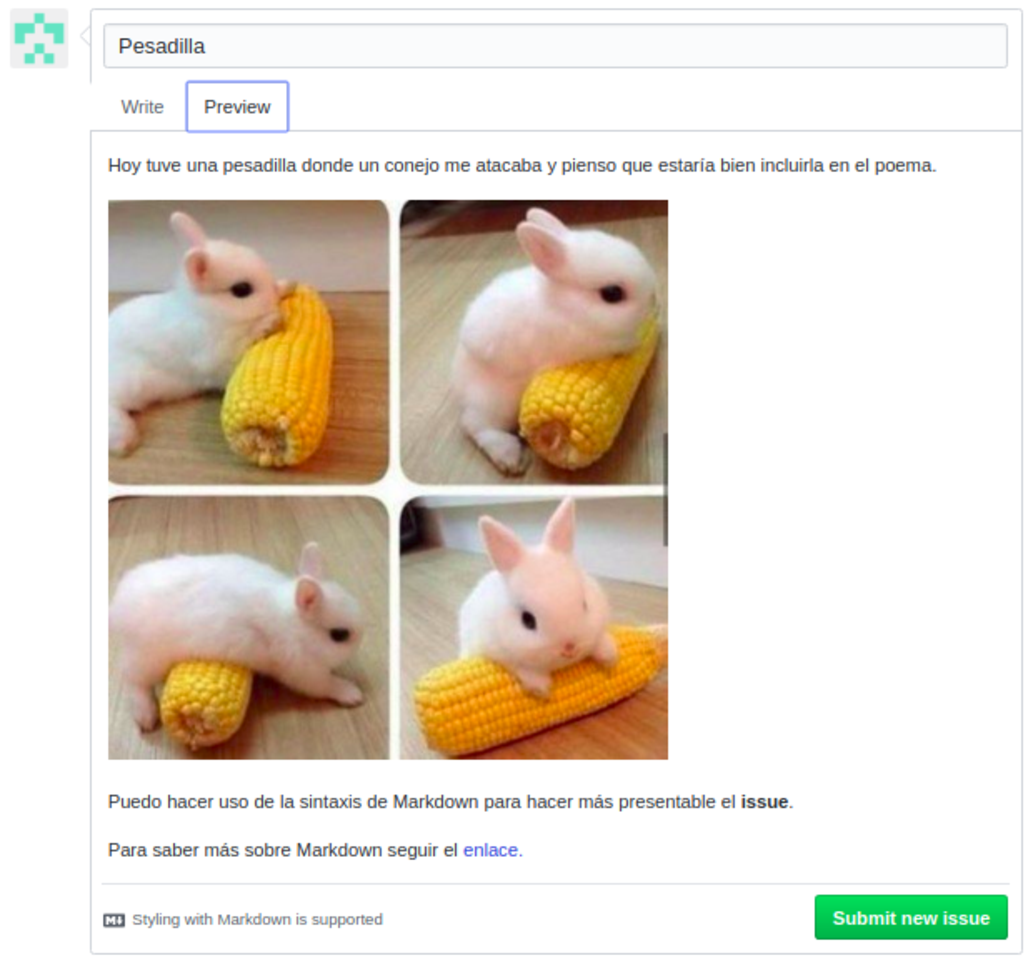
\includegraphics [scale=0.4]{styling}
\label{fig:styling}
\end{figure}
    
\end{block}

\end{frame}

\begin{frame}{Issues}{Problemas con el poema e ideas para mejorarlo}
\begin{block}{Etiquetas y Asignaciones}

\begin{columns}[c]
\column{1.3in}
\vspace{0.2in}
\framebox{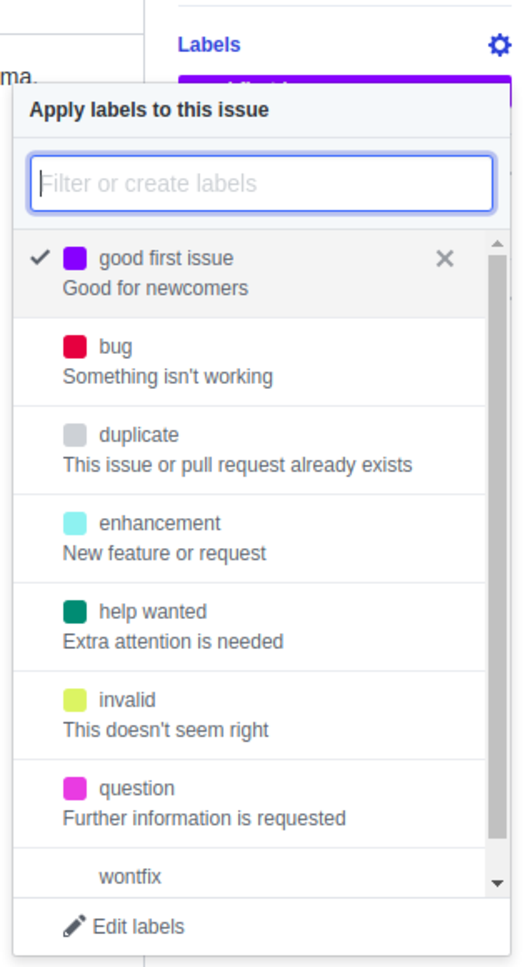
\includegraphics[width=1.3in]{labels}}

\column{1.3in}
\framebox{
\includegraphics[width=1.3in]{assignees}}
\end{columns}
    
\end{block}

\end{frame}

\begin{frame}{Issues}{Problemas con el poema e ideas para mejorarlo}

\begin{block}{}
\vspace{-0.3in}
\begin{figure}[h!]
\centering
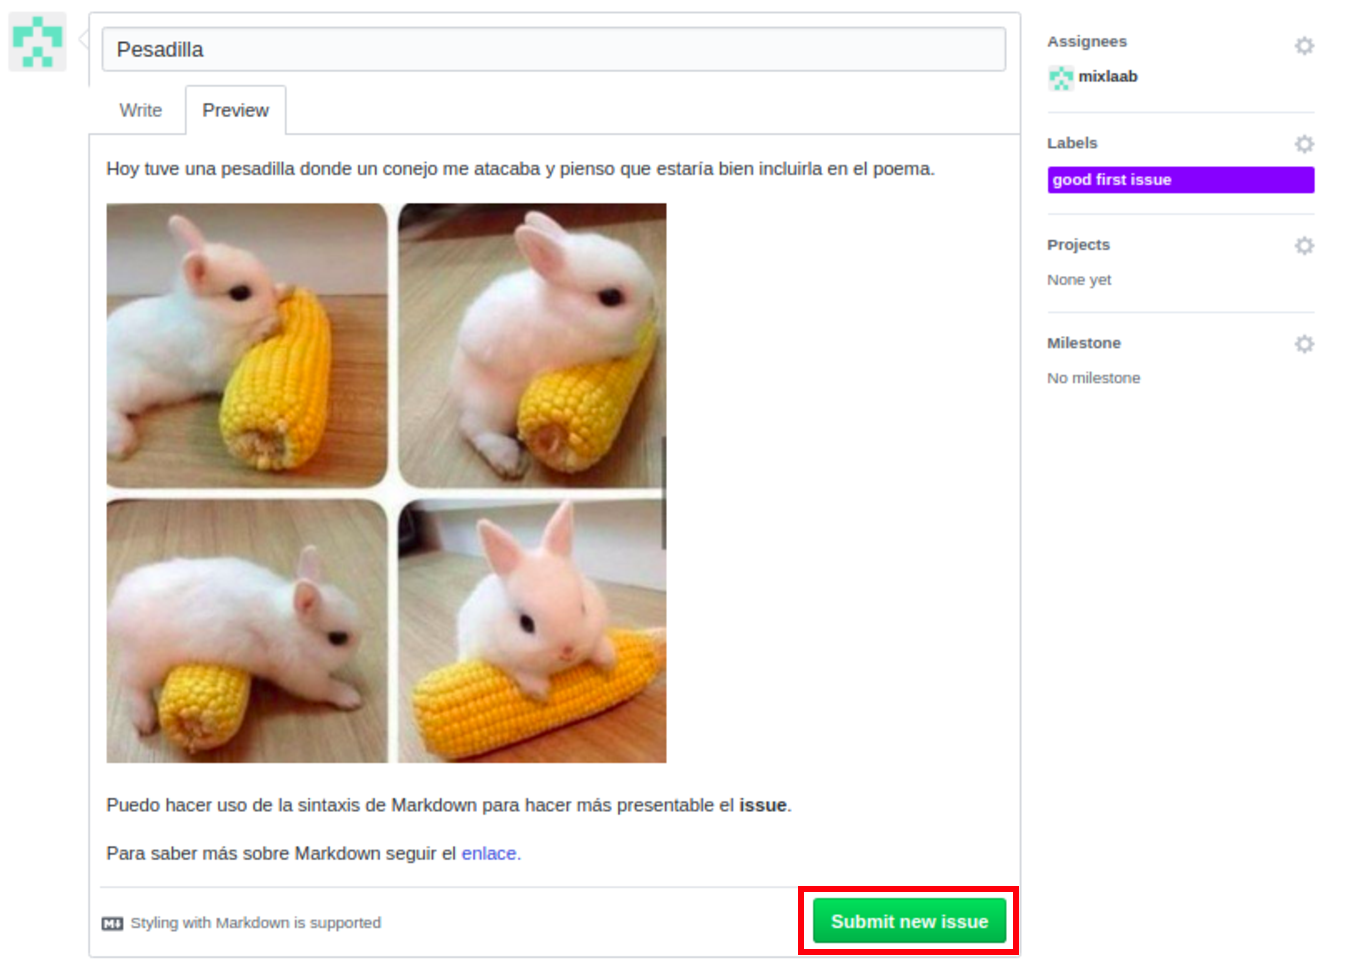
\includegraphics [scale=0.42]{submit}
\label{fig:submit}
\end{figure}
    
\end{block}

\end{frame}

\begin{frame}{Issues}{Problemas con el poema e ideas para mejorarlo}

\begin{block}{Abierto/Cerrado}
Un \textcolor{blue}{issue} permanece abierto hasta que es resuelto. Una vez que el problema ha sido resuelto se dice que el \textcolor{blue}{issue} ha sido cerrado. Cualquiera puede abrir un \textcolor{blue}{issue} en un repositorio.
\vspace{-0.1in}
\begin{figure}[h!]
\centering
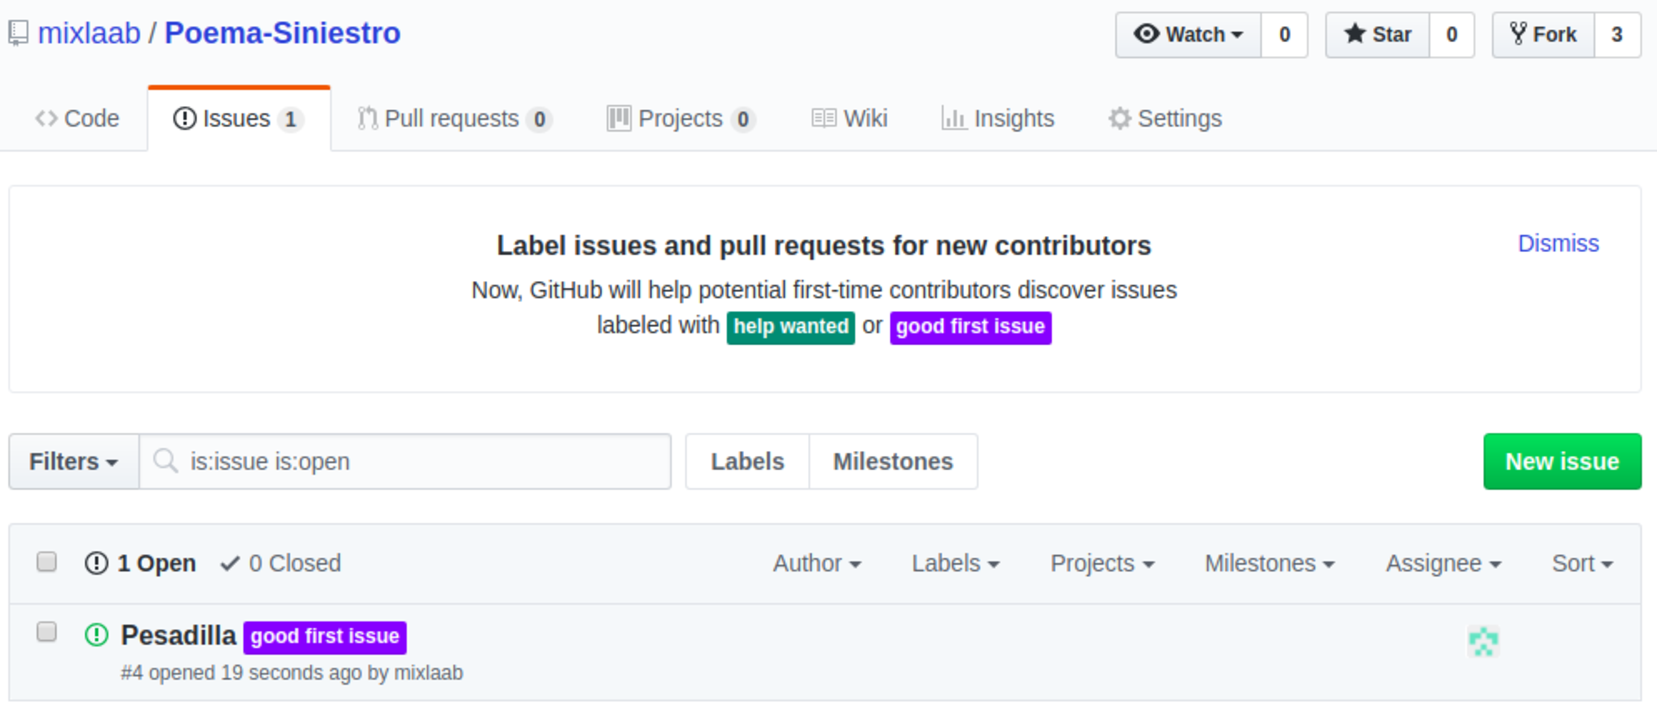
\includegraphics [scale=0.35]{firstissue}
\label{fig:first}
\end{figure}
    
\end{block}

\end{frame}


\begin{frame}{Issues}{Problemas con el poema e ideas para mejorarlo}

\begin{block}{Abierto/Cerrado}
Un \textcolor{blue}{issue} permanece abierto hasta que es resuelto. Una vez que el problema ha sido resuelto se dice que el \textcolor{blue}{issue} ha sido cerrado. Cualquiera puede abrir un \textcolor{blue}{issue} en un repositorio.
\vspace{-0.1in}
\begin{figure}[h!]
\centering
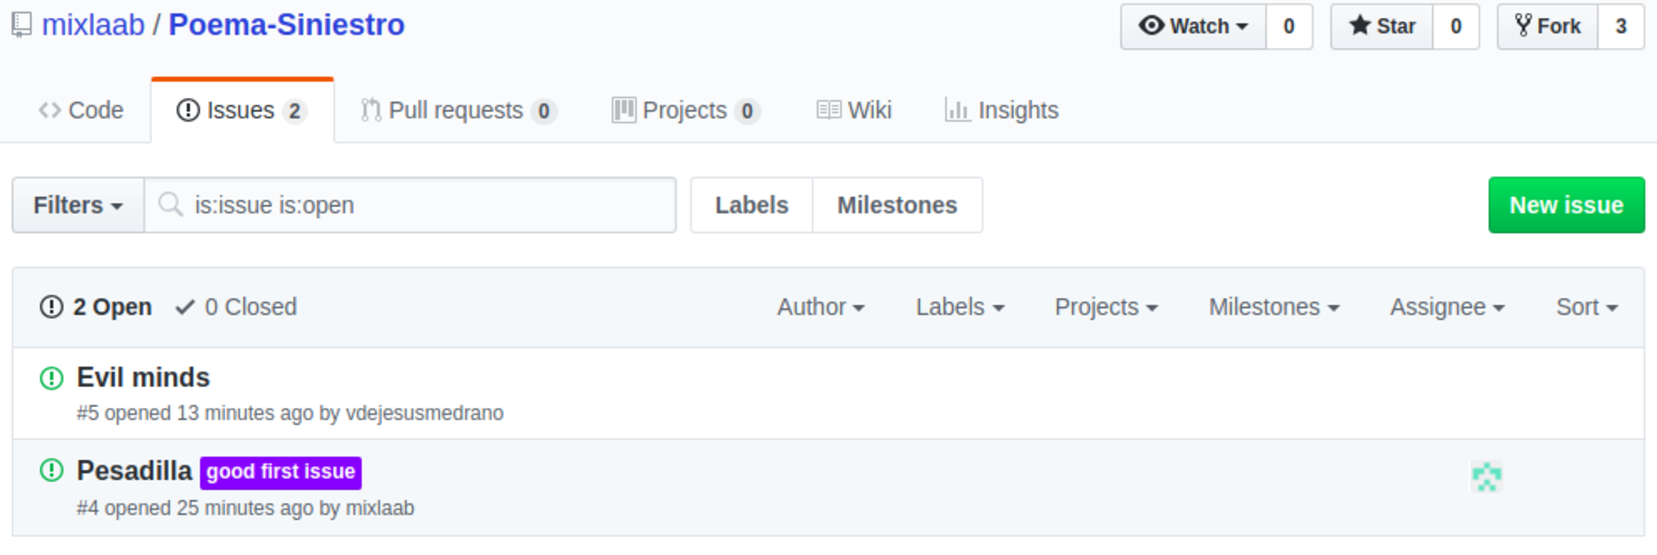
\includegraphics [scale=0.35]{2ndissue}
\label{fig:first}
\end{figure}
    
\end{block}

\end{frame}

\begin{frame}{Issues}{Problemas con el poema e ideas para mejorarlo}

\begin{block}{Resolviendo issues}
Haremos cambios en el poema para resolver el \textcolor{blue}{issue} que hemos abierto. Veremos como hacer referencia a este mismo \textcolor{blue}{issue}.
%\vspace{-0.1in}
\begin{columns}[c]
\column{1.7in}
\vspace{0.2in}
\framebox{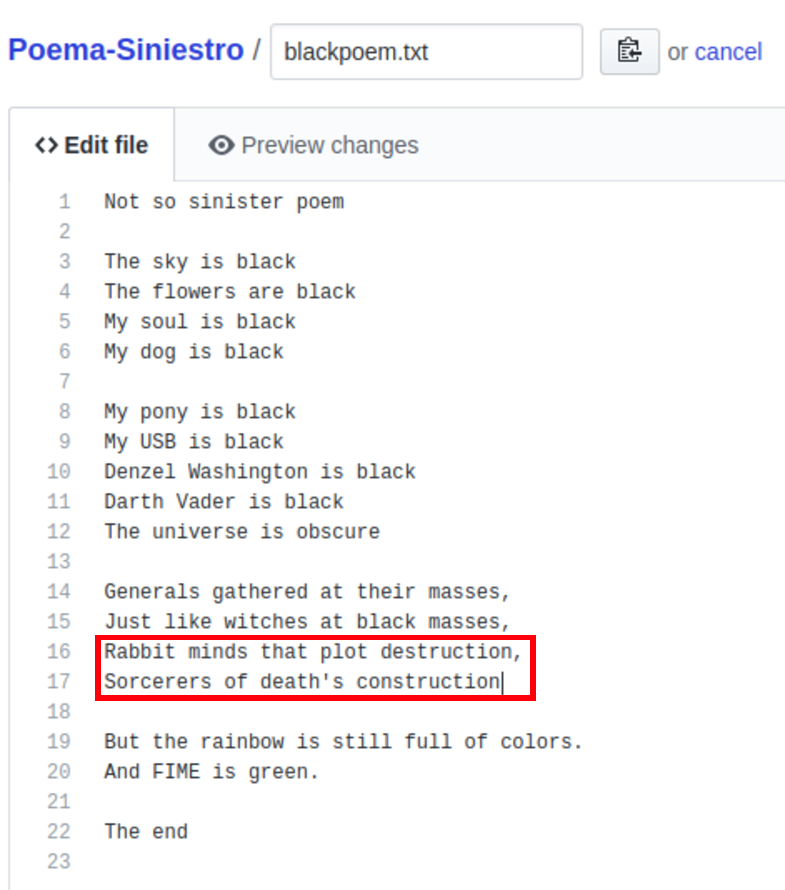
\includegraphics[width=1.7in]{rabbitminds.pdf}}

\column{1.7in}
\framebox{
\includegraphics[width=1.7in]{evilrabbit}}
\end{columns}
    
\end{block}

\end{frame}

\begin{frame}{Issues}{Problemas con el poema e ideas para mejorarlo}

\begin{block}{Referencia a issues}
Al momento de hacer el cambio en el poema podemos hacer referencia al \textcolor{blue}{issue} que estamos tratando de resolver.
\vspace{-0.1in}
\begin{figure}[h!]
\centering
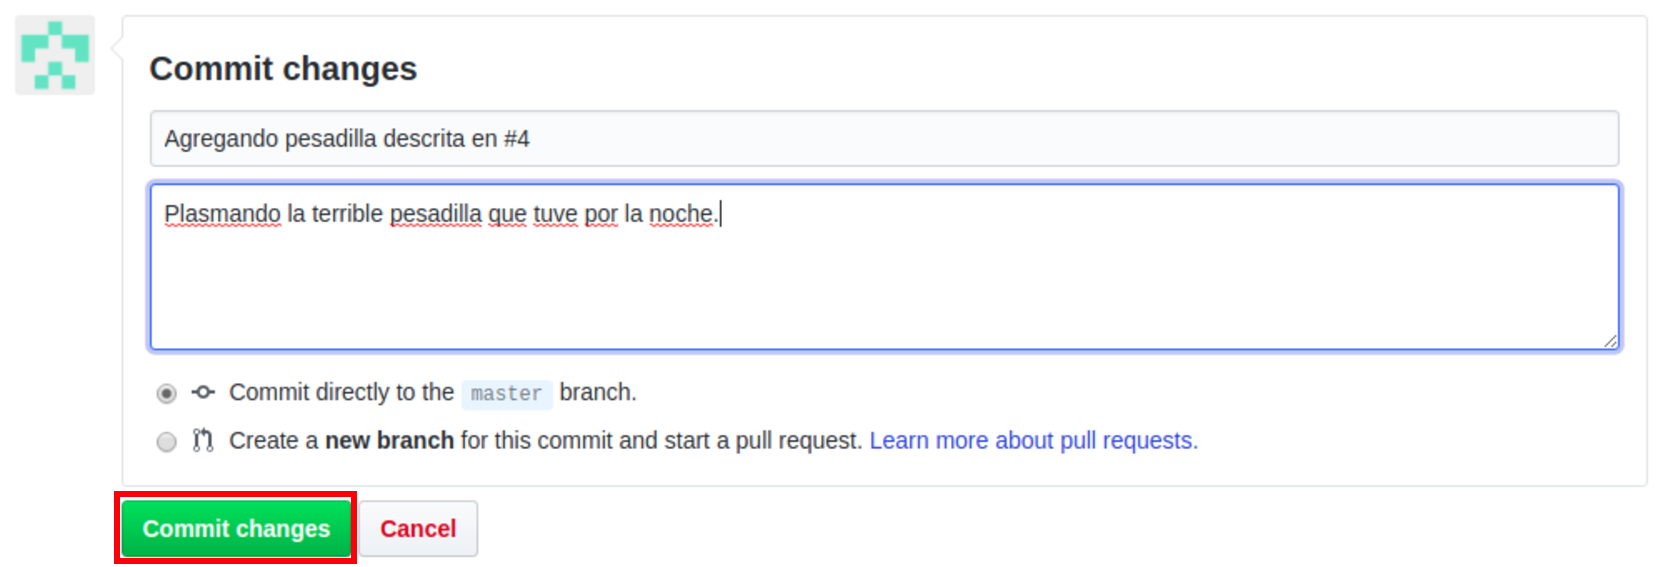
\includegraphics [scale=0.35]{referenceissue}
\label{fig:first}
\end{figure}
    
\end{block}

\end{frame}

\begin{frame}{Issues}{Problemas con el poema e ideas para mejorarlo}

\begin{block}{Referencia a issues}
Una vez haciendo referencia al \textcolor{blue}{issue}, podemos ir a la página de \textcolor{blue}{issues} y dar clic en el \textcolor{blue}{issue} particular al que hemos hecho referencia para ver los cambios en relación a este mismo.

\begin{columns}[c]
\column{1.7in}
%\vspace{0.2in}
\framebox{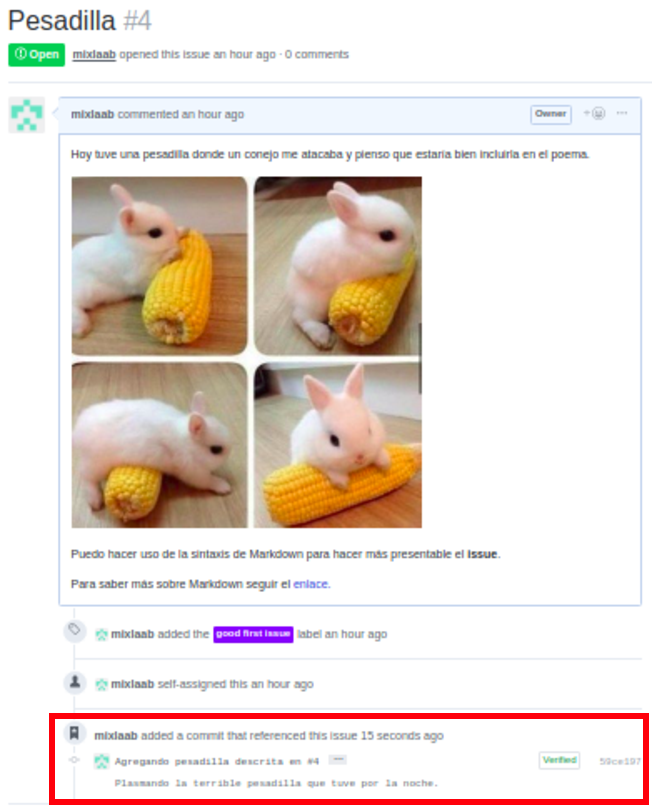
\includegraphics[width=1.7in]{referenceissue2.pdf}}

\column{1.7in}

\framebox{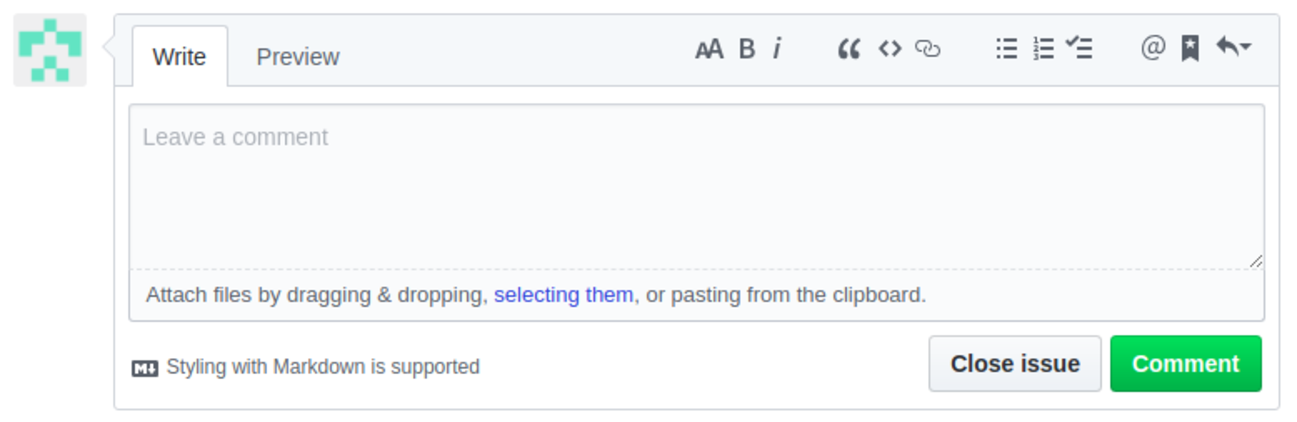
\includegraphics[width=1.7in]{closeissue.pdf}}
\end{columns}
    
\end{block}

\end{frame}

\begin{frame}{Issues}{Problemas con el poema e ideas para mejorarlo}

\begin{block}{Referencia a issues}
Dando clic al cambio hecho nos muestra lo siguiente:
\vspace{-0.1in}
\begin{figure}[h!]
\centering
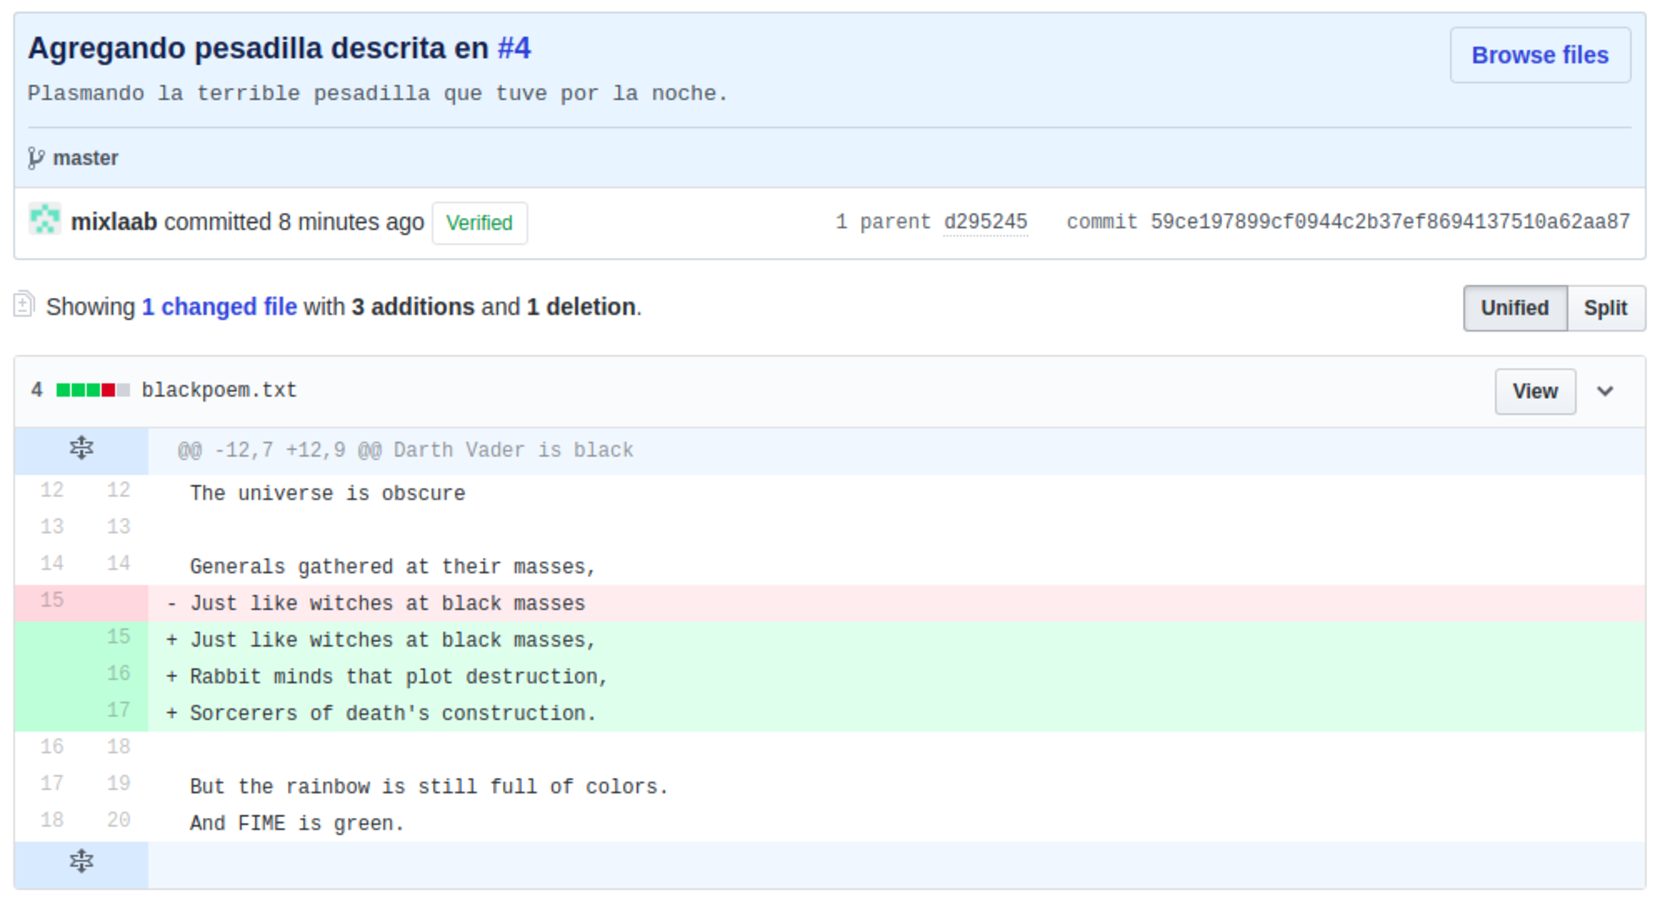
\includegraphics [scale=0.35]{changesissue}
\label{fig:first}
\end{figure}
    
\end{block}

\end{frame}

\begin{frame}{Issues}{Problemas con el poema e ideas para mejorarlo}

\begin{block}{Cerrando issues}
Podemos hacer uso de la palabra clave \textcolor{blue}{fixes} en el titulo del \textcolor{blue}{commit} para cerrar un \textcolor{blue}{issue}.

\begin{columns}[c]
\column{1.2in}
\vspace{0.2in}
\framebox{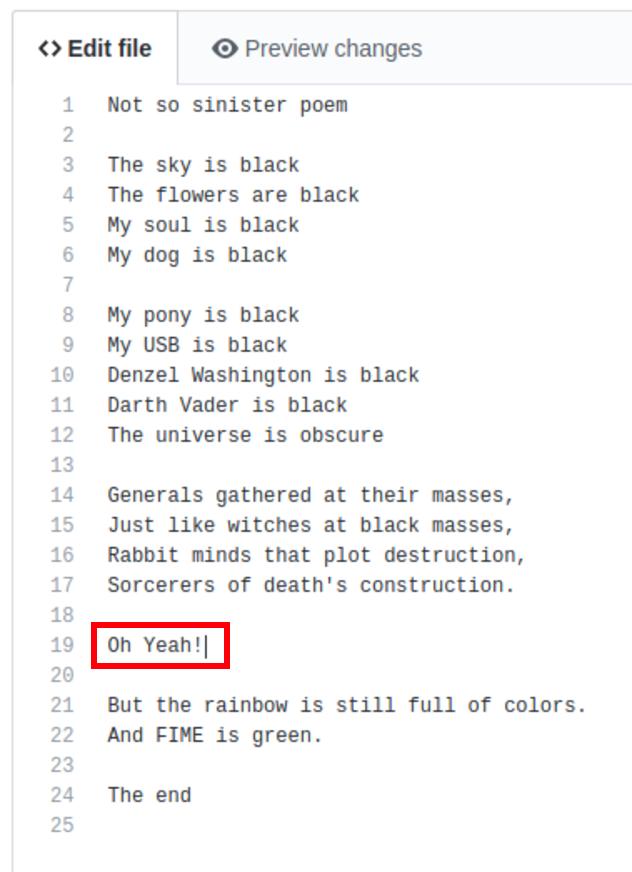
\includegraphics[width=1.2in]{closeissue2.pdf}}

\column{2.2in}

\framebox{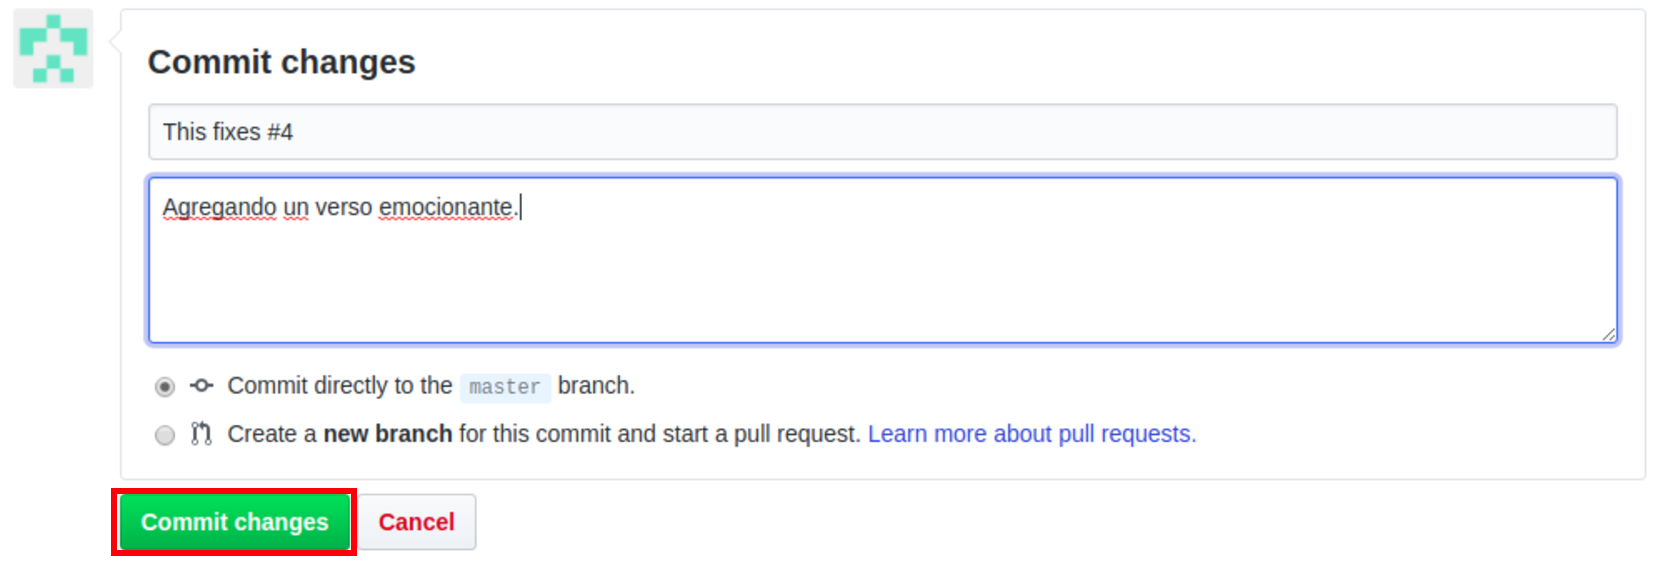
\includegraphics[width=2.2in]{closeissue3.pdf}}
\end{columns}
    
\end{block}

\end{frame}

\begin{frame}{Issues}{Problemas con el poema e ideas para mejorarlo}

\begin{block}{Cerrando issues}
Nos vamos a la página del issue al que hicimos referencia para verificar que ha sido cerrado.
\vspace{-0.1in}
\begin{figure}[h!]
\centering
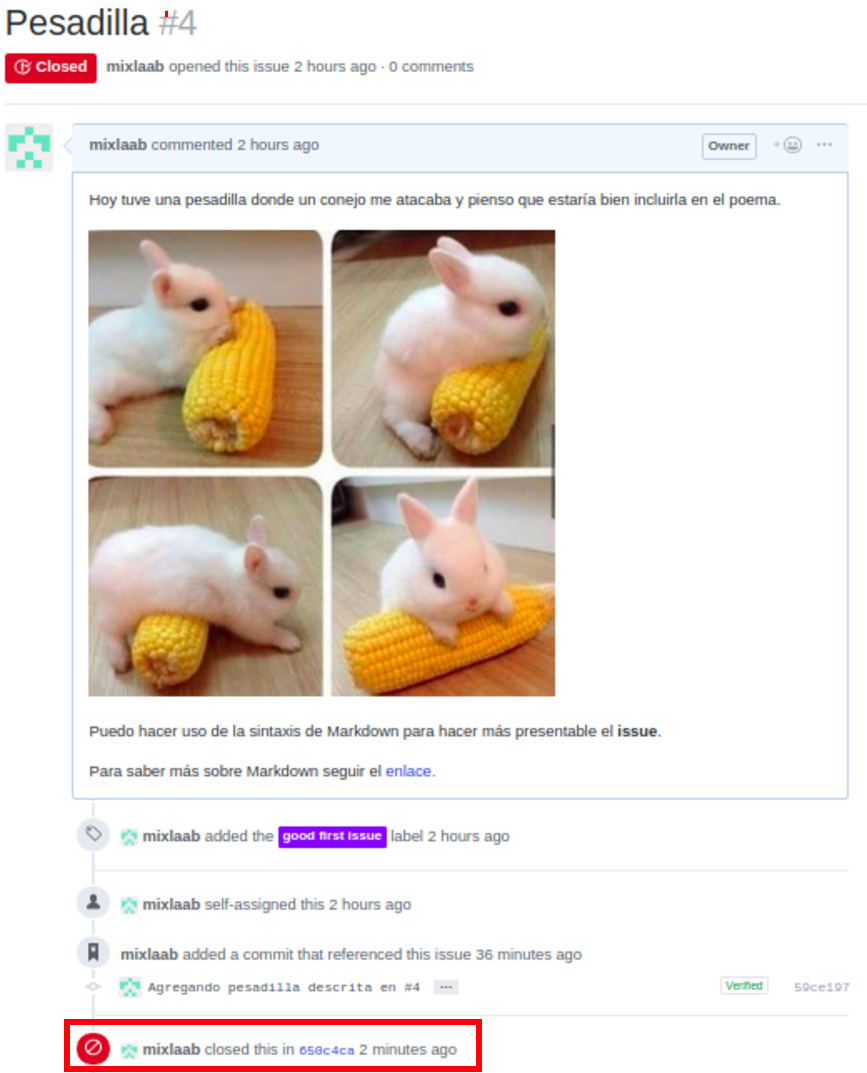
\includegraphics [scale=0.33]{closeissue4}
\label{fig:first}
\end{figure}
    
\end{block}

\end{frame}

\begin{frame}{Issues}{Problemas con el poema e ideas para mejorarlo}

\begin{block}{Referencia a commits}
Iremos a la página de commits para hacer referencia a uno de ellos.
\vspace{0.1in}
\begin{figure}[h!]
\centering
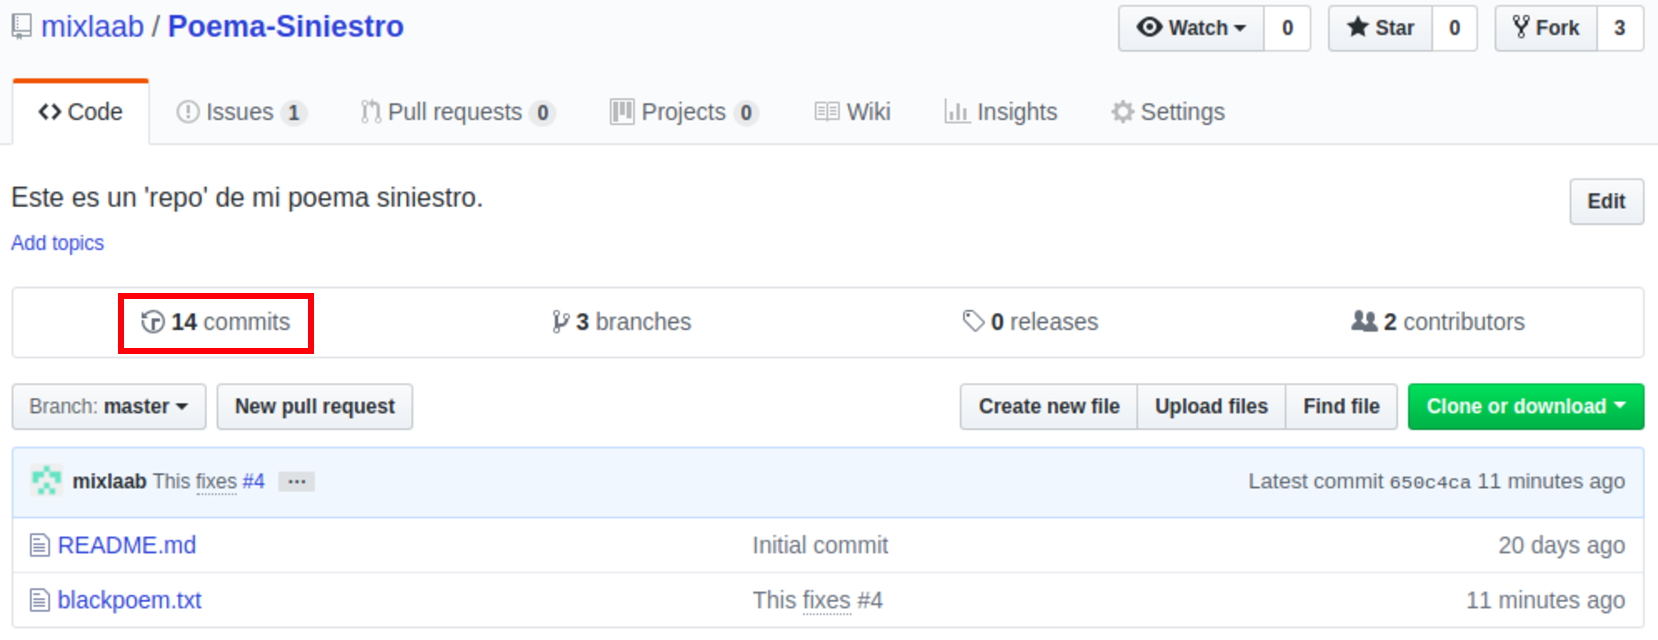
\includegraphics [scale=0.33]{commits}
\label{fig:first}
\end{figure}
    
\end{block}

\end{frame}

\begin{frame}{Issues}{Problemas con el poema e ideas para mejorarlo}

\begin{block}{Referencia a commits}
Daremos clic al que se muestra en la figura.
\vspace{0.1in}
\begin{figure}[h!]
\centering
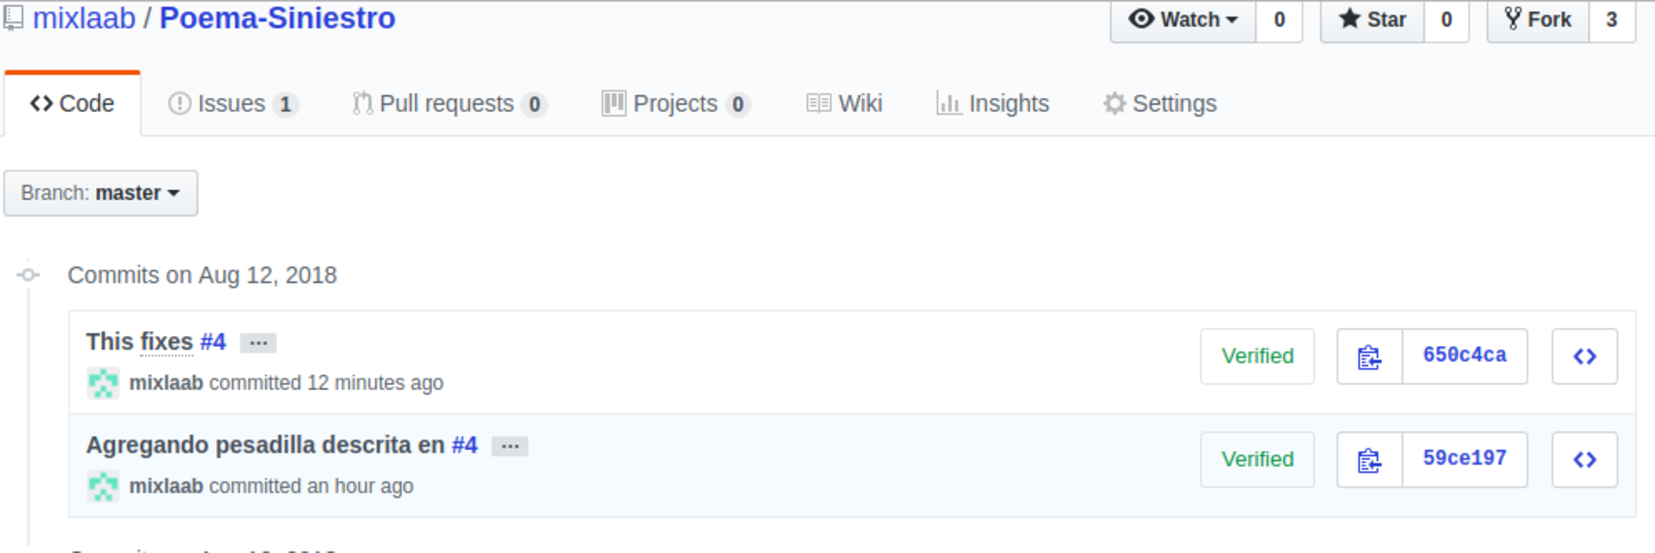
\includegraphics [scale=0.35]{commits2}
\label{fig:first}
\end{figure}
    
\end{block}

\end{frame}

\begin{frame}{Issues}{Problemas con el poema e ideas para mejorarlo}

\begin{block}{Referencia a commits}
Copiaremos el commit hash.
\vspace{0.1in}
\begin{figure}[h!]
\centering

\includegraphics [scale=0.35]{commithash}
\label{fig:first}
\end{figure}
    
\end{block}

\end{frame}

\begin{frame}{Issues}{Problemas con el poema e ideas para mejorarlo}

\begin{block}{Referencia a commits}
\vspace{0.1in}
\begin{figure}[h!]
\centering
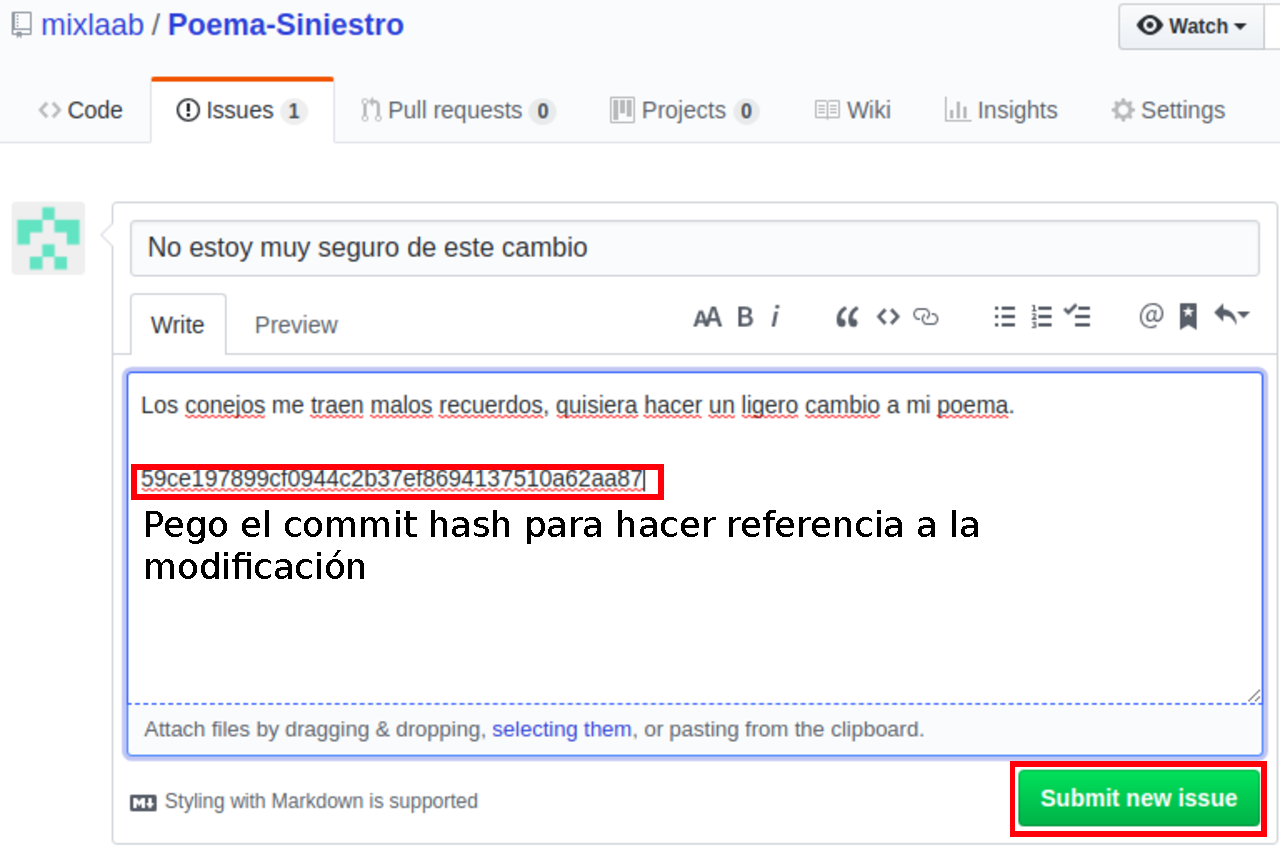
\includegraphics [scale=0.35]{commitreference}
\label{fig:first}
\end{figure}
    
\end{block}

\end{frame}

\begin{frame}{Issues}{Problemas con el poema e ideas para mejorarlo}

\begin{block}{Referencia a commits}
Se ha creado un \textcolor{blue}{issue} haciendo referencia a un \textcolor{blue}{commit}.
\vspace{0.1in}
\begin{figure}[h!]
\centering

\includegraphics [scale=0.42]{commitreference2}
\label{fig:first}
\end{figure}
    
\end{block}

\end{frame}
%%%%%%%%%%%%%%%%%%%%%%%%%%%%

\section{Tarea}
\begin{frame}{Tarea}{Aplicando el concepto de issues}

\begin{block}{Tarea #3}
En equipo realizar las siguientes actividades:
\vspace{0.1in}
\begin{itemize}
    \item El líder de cada equipo creará un repositorio llamado MateriaHoraEquipo\_\#.
    \item El líder escribirá la estrofa de un poema y creará tres issues haciendo uso de etiquetas (labels) y asignando uno distinto a cada miembro del equipo (incluido a sí mismo).
    \item Cada miembro del equipo deberá resolver uno de los issues que el líder ha creado y hacer un pull request al líder para incluir la mejora. Los issues deberán cerrarse.
    \item Se adjunta un archivo .txt con el enlace al repositorio, una vez que se hayan seguido todos los pasos.
\end{itemize}
    
\end{block}

\end{frame}

\section{Información de contacto}
% contact information
\begin{frame}{Feedback}{Información de contacto}
En caso de comentarios, sugerencias, preguntas o errores en las diapositivas no dudes en contactarme.
  \begin{center}
    \insertauthor\\
    \chref{https://mixlaab.github.io}{https://mixlaab.github.io}\\
    WA: 8119022700\\
    %9220 Aalborg Ø
  \end{center}
\end{frame}
%%%%%%%%%%%%%%%%

{\aauwavesbg%
\begin{frame}[plain,noframenumbering]%
  \finalpage{Fin}
\end{frame}}
%%%%%%%%%%%%%%%%

\end{document}
